\documentclass[journal,12pt,twocolumn]{IEEEtran}
\usepackage[cmex10]{amsmath}
\usepackage{graphicx}
\usepackage[font=normal]{caption}

%\usepackage{pgfplots}
%\pgfplotsset{compat=newest}
%\pgfplotsset{scaled y ticks=false}
%\usepgfplotslibrary{groupplots}
%\usepgfplotslibrary{dateplot}
%
%\usepackage{tikz}
%
%\pgfplotsset{compat=1.11,
% /pgfplots/ybar legend/.style={
% /pgfplots/legend image code/.code={
% \draw[##1,/tikz/.cd,yshift=-0.25em]
% (0cm,0cm) rectangle (3pt,0.8em);},
% },
%}

\let\vec\mathbf
\newcommand{\myvec}[1]{\ensuremath{\begin{pmatrix}#1\end{pmatrix}}}
\newcommand{\mydet}[1]{\ensuremath{\begin{vmatrix}#1\end{vmatrix}}}
\providecommand{\brak}[1]{\ensuremath{\left(#1\right)}}
\providecommand{\norm}[1]{\left\lVert#1\right\rVert}
\newcommand\numberthis{\addtocounter{equation}{1}\tag{\theequation}}
\providecommand{\abs}[1]{\left\vert#1\right\vert}
\providecommand{\lbrak}[1]{\ensuremath{\left(#1\right.}}
\providecommand{\rbrak}[1]{\ensuremath{\left.#1\right)}}
\providecommand{\sbrak}[1]{\ensuremath{{}\left[#1\right]}}


\title{Conic section using Python}
\author{Ahilan R - FWC22090}

\begin{document}
\maketitle

\subsection*{\textbf{Problem}}
Find the equation of the common tangent to the curves 
\begin{align}
		y^2&=8x \label{eq:parab} \\
		xy&=-1 \label{eq:hyp}
\end{align}
\subsection*{\textbf{Solution}}
\eqref{eq:parab} and \eqref{eq:hyp} can be expressed in vector forms
\begin{align}
		\vec{x}^{\top}\vec{V_1}\vec{x} + 2\vec{u_1}^{\top}\vec{x} + f_1 &= 0  \label{eq:par} \\
		\vec{x}^{\top}\vec{V_2}\vec{x}  + 2\vec{u_2}^{\top}\vec{x} + f_2 &= 0 \label{eq:hi} 
\end{align}
where,
\begin{align}
		\vec{V_1} &= \myvec{0&0\\0&1} \text{,}\quad  
		\vec{u_1} = \myvec{-8\\0}  \text{,} \quad  f_1 = 0\\
		\vec{V_2} &= \myvec{0&\frac{1}{2}\\\frac{1}{2}&0} \text{,} \quad 
		  \vec{u_2} = \myvec{0\\0} \text{,}  \quad f_2 = 1 \text{.} %\quad \text{and}
\end{align}
\\
In projective plane \eqref{eq:par} and \eqref{eq:hi} becomes %are represented by
\begin{align}
		\vec{X}^{\top}\vec{M_1}\vec{X} &= 0 \label{eq:ppar} \\
		\vec{X}^{\top}\vec{M_2}\vec{X} &= 0 \label{eq:phi} 
\end{align}
where,
\begin{align}
		\vec{M_1} &= \myvec{\vec{V_1}&\vec{u_1}\\\vec{u_1}^{\top}&f_1} \text{, } \\[0.5ex]
		\vec{M_2} &= \myvec{\vec{V_2}&\vec{u_2}\\\vec{u_2}^{\top}&f_2} \text{,} \text{ and } 
		\vec{X}=\myvec{\vec{x}\\1} 
\end{align}
Here, $\vec{M_1}$ and $\vec{M_2}$ are symmetric, and $\vec{X}$ is called the homogeneous coordinate of $\vec{x}$. \\
The dual conics of \eqref{eq:ppar} and \eqref{eq:phi} is given by
\begin{align}
		\vec{X}^{\top}\mydet{\vec{M_1}}\vec{M_1^{-1}}\vec{X} &= 0 \label{eq:pd} \\
		\vec{X}^{\top}\mydet{\vec{M_2}}\vec{M_2^{-1}}\vec{X} &= 0 \label{eq:hd} 
\end{align}
The dual conics \eqref{eq:pd} and \eqref{eq:hd} intersect at most at 4 points $\vec{x_i}$. The corresponding common tangent(s) is given by \[ \myvec{\vec{x_i}^{\top}&1}\vec{X}=0 \label{eq:tangent_eqn} \numberthis \]
\begin{align}
		\mydet{\vec{M_1}}\vec{M_1^{-1}} &\text{ can be written as } \myvec{\vec{N_1}&\vec{w_1}\\\vec{w_1}^{\top}&k_1} \\[0.5ex]
		\mydet{\vec{M_2}}\vec{M_2^{-1}} &\text{ can be written as } \myvec{\vec{N_2}&\vec{w_2}\\\vec{w_2}^{\top}&k_2}
\end{align}
Let's take, 
\begin{align}
		\vec{N} = \vec{N_1}+\mu\vec{N_2} \quad \text{and} \quad
		\vec{w} = \vec{w_1}+\mu\vec{w_2} \text{.}
\end{align}
\\
The intersection of dual conics is given by
\begin{align}
\mydet{\vec{M_1}}\vec{M_1^{-1}}+\mu\mydet{\vec{M_2}}\vec{M_2^{-1}} = 0 \label{eq:dual_intersect}
\end{align}
The intersection \eqref{eq:dual_intersect} represents a pair of straight lines if 
\begin{gather}
		\mydet{\mydet{\vec{M_1}}\vec{M_1^{-1}}+\mu\mydet{\vec{M_2}}\vec{M_2^{-1}}} = 0 \\
	\text{and }	\mydet{\vec{N_1}+\mu\vec{N_2}} < 0	
\end{gather}
On solving, we get $\mu=-16$. % Substituting $\mu$ in \eqref{eq:dual_intersect}, we get 
The point of intersection of two lines of the pair of straight lines represented by \eqref{eq:dual_intersect}, point $H$, is given by %The center of the pair of straight lines given by \eqref{eq:dual_intersect} is  
\begin{equation}
		\vec{h} = -\vec{N}^{-1}\vec{w} %-\brak{\vec{N_1}+\mu\vec{N_2}}^{-1}\brak{\vec{w_1}+\mu\vec{w_2}}
\end{equation}
The normal vectors of the two lines of \eqref{eq:dual_intersect} are given by
\begin{align}
		\vec{n_1} &= \vec{P}\myvec{\sqrt{\abs{\lambda_1}}\\ \sqrt{\abs{\lambda_2}}} \text{ and } \\
		\vec{n_2} &= \vec{P}\myvec{\sqrt{\abs{\lambda_1}}\\ -\sqrt{\abs{\lambda_2}}}
\end{align}
where $\lambda_i, \vec{P}$ are the eigenparameters of $\vec{N}$. Then, the direction vectors of lines of \eqref{eq:dual_intersect} are given by
\begin{gather}
		\vec{m_1} = \vec{R}_{\frac{\pi}{2}}\vec{n_1} \text{ and } \vec{m_2} = \vec{R}_{\frac{\pi}{2}}\vec{n_2}
\end{gather}
where, \[ \vec{R}_{\theta} = \myvec{\cos  \theta & -\sin \theta \\ \sin \theta & \cos \theta} \text{.} \]
Therefore, the lines of \eqref{eq:dual_intersect} are given by
\begin{align}
		\vec{x} = \vec{h} + \kappa\vec{m_1} \quad \text{and} \quad
		\vec{x} = \vec{h} + \kappa\vec{m_2} 
\end{align}
\newpage
The points of intersection of the lines $\vec{x} = \vec{h} + \kappa\vec{m_k}$ with a dual conic, say $\vec{X}^{\top}\mydet{\vec{M_1}}\vec{M_1^{-1}}\vec{X}$, which are also the point(s) intersection of the dual conics, are given by
\begin{align}
		\vec{x_i} = \vec{h} + \kappa_j\vec{m_k}
\end{align}
where,
{\tiny
\begin{multline}
\kappa_j = \frac{1}
{
\vec{m_1}^T\vec{N_1}\vec{m_1}
}
\lbrak{-\vec{m_1}^{\top}\brak{\vec{N_1}\vec{h}+\vec{w_1}}}
\\[0.5ex]
\pm
\rbrak{\sqrt{
\sbrak{
\vec{m_1}^{\top}\brak{\vec{N_1}\vec{h}+\vec{w_1}}
}^2
-
\brak
{
\vec{h}^{\top}\vec{N_1}\vec{h} + 2\vec{w_1}^{\top}\vec{h} +k_1
}
\brak{\vec{m_1}^{\top}\vec{N_1}\vec{m_1}}
}
}
\end{multline}
}
\vspace{-0.5cm}
\begin{figure}[h]
\centering
%\def\figwidth{\linewidth}
%\def\figheight{0.35\textheight} % Feel free to change
%% This file was created with tikzplotlib v0.10.1.
\begin{tikzpicture}

\definecolor{darkgray176}{RGB}{176,176,176}
\definecolor{lightgray204}{RGB}{204,204,204}
\definecolor{purple}{RGB}{128,0,128}

\begin{axis}[
height=\figheight,
legend cell align={left},
legend style={fill opacity=0.8, draw opacity=1, text opacity=1, draw=lightgray204},
tick align=outside,
tick pos=left,
width=\figwidth,
x grid style={darkgray176},
xlabel={\(\displaystyle X\)},
xmajorgrids,
xmin=-2.22380952380953, xmax=7.22380952380953,
xtick style={color=black},
y grid style={darkgray176},
ylabel style={rotate=-90.0},
ylabel={\(\displaystyle Y\)},
ymajorgrids,
ymin=-0.52, ymax=6.52,
ytick style={color=black}
]
\addplot [semithick, black, forget plot]
table {%
2 1
2.11111111111111 1
2.22222222222222 1
2.33333333333333 1
2.44444444444444 1
2.55555555555556 1
2.66666666666667 1
2.77777777777778 1
2.88888888888889 1
3 1
};
\addplot [semithick, black, forget plot]
table {%
3 1
3 1.44444444444444
3 1.88888888888889
3 2.33333333333333
3 2.77777777777778
3 3.22222222222222
3 3.66666666666667
3 4.11111111111111
3 4.55555555555556
3 5
};
\addplot [semithick, black, forget plot]
table {%
3 5
2.88888888888889 5
2.77777777777778 5
2.66666666666667 5
2.55555555555556 5
2.44444444444444 5
2.33333333333333 5
2.22222222222222 5
2.11111111111111 5
2 5
};
\addplot [semithick, black, forget plot]
table {%
2 5
2 4.55555555555556
2 4.11111111111111
2 3.66666666666667
2 3.22222222222222
2 2.77777777777778
2 2.33333333333333
2 1.88888888888889
2 1.44444444444444
2 1
};
\addplot [semithick, purple, dashed]
table {%
3.1 5.4
2.96666666666667 4.86666666666667
2.83333333333333 4.33333333333333
2.7 3.8
2.56666666666667 3.26666666666667
2.43333333333333 2.73333333333333
2.3 2.2
2.16666666666667 1.66666666666667
2.03333333333333 1.13333333333333
1.9 0.6
};
\addlegendentry{$Diag 1$}
\addplot [semithick, blue, dashed]
table {%
1.9 5.4
2.03333333333333 4.86666666666667
2.16666666666667 4.33333333333333
2.3 3.8
2.43333333333333 3.26666666666667
2.56666666666667 2.73333333333333
2.7 2.2
2.83333333333333 1.66666666666667
2.96666666666667 1.13333333333333
3.1 0.6
};
\addlegendentry{$Diag 2$}
\addplot [semithick, black, dashed, forget plot]
table {%
2 6.2
2 5.48888888888889
2 4.77777777777778
2 4.06666666666667
2 3.35555555555556
2 2.64444444444444
2 1.93333333333333
2 1.22222222222222
2 0.511111111111111
2 -0.2
};
\addplot [semithick, black, dashed, forget plot]
table {%
4.2 1
3.82222222222222 1
3.44444444444444 1
3.06666666666667 1
2.68888888888889 1
2.31111111111111 1
1.93333333333333 1
1.55555555555556 1
1.17777777777778 1
0.8 1
};
\addplot [semithick, black, dashed, forget plot]
table {%
3 6.2
3 5.48888888888889
3 4.77777777777778
3 4.06666666666667
3 3.35555555555556
3 2.64444444444444
3 1.93333333333333
3 1.22222222222222
3 0.511111111111111
3 -0.2
};
\addplot [semithick, black, dashed, forget plot]
table {%
4.2 5
3.82222222222222 5
3.44444444444444 5
3.06666666666667 5
2.68888888888889 5
2.31111111111111 5
1.93333333333333 5
1.55555555555556 5
1.17777777777778 5
0.8 5
};
\draw (axis cs:2.01,0.7) node[
  scale=0.5,
  anchor=base west,
  text=black,
  rotate=0.0
]{A};
\draw (axis cs:3.02,0.7) node[
  scale=0.5,
  anchor=base west,
  text=black,
  rotate=0.0
]{B};
\draw (axis cs:2.02,5.08) node[
  scale=0.5,
  anchor=base west,
  text=black,
  rotate=0.0
]{D};
\draw (axis cs:3.02,5.08) node[
  scale=0.5,
  anchor=base west,
  text=black,
  rotate=0.0
]{C};
\draw (axis cs:1.6,0) node[
  scale=0.5,
  anchor=base west,
  text=black,
  rotate=0.0
]{$L_1$};
\draw (axis cs:1,1.2) node[
  scale=0.5,
  anchor=base west,
  text=black,
  rotate=0.0
]{$L_2$};
\draw (axis cs:3.2,6) node[
  scale=0.5,
  anchor=base west,
  text=black,
  rotate=0.0
]{$L_3$};
\draw (axis cs:1,5.2) node[
  scale=0.5,
  anchor=base west,
  text=black,
  rotate=0.0
]{$L_4$};
\end{axis}

\end{tikzpicture}

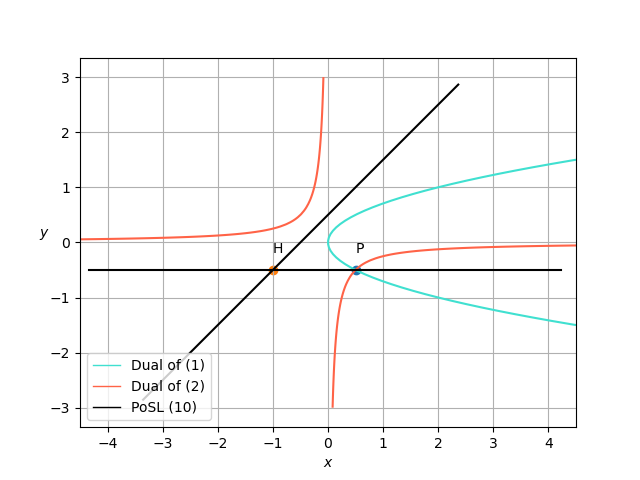
\includegraphics[width=\columnwidth]{figs/dual_int.png}
\label{fig:dual_int}
\caption{Intersection of the Dual Curves}
\end{figure}

Upon substituting respective values we find that the dual conics \eqref{eq:pd} and \eqref{eq:hd} inersect at a single point, $P=\vec{p}=\myvec{0.5\\-0.5}$. 
\\[0.7ex]
Then from \eqref{eq:tangent_eqn}, 
\begin{align}
		\myvec{\vec{p}^{\top}&1}\vec{X} &= 0 \\
		\vec{p}^{\top}\vec{x} + 1 &= 0 \\
		\myvec{0.5&-0.5}\vec{x} &= -1 \label{eq:comm_tang} \numberthis
\end{align}
Thus, \eqref{eq:comm_tang} is the equation of common tangent to the curves \eqref{eq:parab} and \eqref{eq:hyp}.
\newpage

\begin{figure}[h!]
\centering
%\def\figwidth{\linewidth}
%\def\figheight{0.35\textheight} % Feel free to change
%% This file was created with tikzplotlib v0.10.1.
\begin{tikzpicture}

\definecolor{darkgray176}{RGB}{176,176,176}
\definecolor{lightgray204}{RGB}{204,204,204}
\definecolor{purple}{RGB}{128,0,128}

\begin{axis}[
height=\figheight,
legend cell align={left},
legend style={fill opacity=0.8, draw opacity=1, text opacity=1, draw=lightgray204},
tick align=outside,
tick pos=left,
width=\figwidth,
x grid style={darkgray176},
xlabel={\(\displaystyle X\)},
xmajorgrids,
xmin=-2.22380952380953, xmax=7.22380952380953,
xtick style={color=black},
y grid style={darkgray176},
ylabel style={rotate=-90.0},
ylabel={\(\displaystyle Y\)},
ymajorgrids,
ymin=-0.52, ymax=6.52,
ytick style={color=black}
]
\addplot [semithick, black, forget plot]
table {%
2 1
2.11111111111111 1
2.22222222222222 1
2.33333333333333 1
2.44444444444444 1
2.55555555555556 1
2.66666666666667 1
2.77777777777778 1
2.88888888888889 1
3 1
};
\addplot [semithick, black, forget plot]
table {%
3 1
3 1.44444444444444
3 1.88888888888889
3 2.33333333333333
3 2.77777777777778
3 3.22222222222222
3 3.66666666666667
3 4.11111111111111
3 4.55555555555556
3 5
};
\addplot [semithick, black, forget plot]
table {%
3 5
2.88888888888889 5
2.77777777777778 5
2.66666666666667 5
2.55555555555556 5
2.44444444444444 5
2.33333333333333 5
2.22222222222222 5
2.11111111111111 5
2 5
};
\addplot [semithick, black, forget plot]
table {%
2 5
2 4.55555555555556
2 4.11111111111111
2 3.66666666666667
2 3.22222222222222
2 2.77777777777778
2 2.33333333333333
2 1.88888888888889
2 1.44444444444444
2 1
};
\addplot [semithick, purple, dashed]
table {%
3.1 5.4
2.96666666666667 4.86666666666667
2.83333333333333 4.33333333333333
2.7 3.8
2.56666666666667 3.26666666666667
2.43333333333333 2.73333333333333
2.3 2.2
2.16666666666667 1.66666666666667
2.03333333333333 1.13333333333333
1.9 0.6
};
\addlegendentry{$Diag 1$}
\addplot [semithick, blue, dashed]
table {%
1.9 5.4
2.03333333333333 4.86666666666667
2.16666666666667 4.33333333333333
2.3 3.8
2.43333333333333 3.26666666666667
2.56666666666667 2.73333333333333
2.7 2.2
2.83333333333333 1.66666666666667
2.96666666666667 1.13333333333333
3.1 0.6
};
\addlegendentry{$Diag 2$}
\addplot [semithick, black, dashed, forget plot]
table {%
2 6.2
2 5.48888888888889
2 4.77777777777778
2 4.06666666666667
2 3.35555555555556
2 2.64444444444444
2 1.93333333333333
2 1.22222222222222
2 0.511111111111111
2 -0.2
};
\addplot [semithick, black, dashed, forget plot]
table {%
4.2 1
3.82222222222222 1
3.44444444444444 1
3.06666666666667 1
2.68888888888889 1
2.31111111111111 1
1.93333333333333 1
1.55555555555556 1
1.17777777777778 1
0.8 1
};
\addplot [semithick, black, dashed, forget plot]
table {%
3 6.2
3 5.48888888888889
3 4.77777777777778
3 4.06666666666667
3 3.35555555555556
3 2.64444444444444
3 1.93333333333333
3 1.22222222222222
3 0.511111111111111
3 -0.2
};
\addplot [semithick, black, dashed, forget plot]
table {%
4.2 5
3.82222222222222 5
3.44444444444444 5
3.06666666666667 5
2.68888888888889 5
2.31111111111111 5
1.93333333333333 5
1.55555555555556 5
1.17777777777778 5
0.8 5
};
\draw (axis cs:2.01,0.7) node[
  scale=0.5,
  anchor=base west,
  text=black,
  rotate=0.0
]{A};
\draw (axis cs:3.02,0.7) node[
  scale=0.5,
  anchor=base west,
  text=black,
  rotate=0.0
]{B};
\draw (axis cs:2.02,5.08) node[
  scale=0.5,
  anchor=base west,
  text=black,
  rotate=0.0
]{D};
\draw (axis cs:3.02,5.08) node[
  scale=0.5,
  anchor=base west,
  text=black,
  rotate=0.0
]{C};
\draw (axis cs:1.6,0) node[
  scale=0.5,
  anchor=base west,
  text=black,
  rotate=0.0
]{$L_1$};
\draw (axis cs:1,1.2) node[
  scale=0.5,
  anchor=base west,
  text=black,
  rotate=0.0
]{$L_2$};
\draw (axis cs:3.2,6) node[
  scale=0.5,
  anchor=base west,
  text=black,
  rotate=0.0
]{$L_3$};
\draw (axis cs:1,5.2) node[
  scale=0.5,
  anchor=base west,
  text=black,
  rotate=0.0
]{$L_4$};
\end{axis}

\end{tikzpicture}

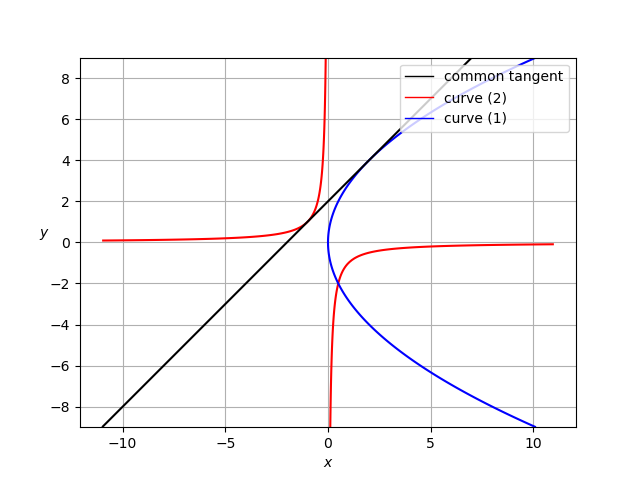
\includegraphics[width=\columnwidth]{figs/comm_tan.png}
\label{fig:comm_tan}
\caption{Common tangent to the given curves}
\end{figure}
\end{document}
